%%%%%%%%%%%%%%%%%%%%%%%%%%%%%%%%%%%%%%%
\section{Estimation Theory}
\label{sec:SDT}
%%%%%%%%%%%%%%%%%%%%%%%%%%%%%%%%%%%%%%%

Estimation theory plays a central role in many data science applications by providing foundational methods for inferring unknown parameters from observed data. Estimation techniques are used to design algorithms that learn from data and make predictions about unseen samples. In signal processing, it helps recover signals from noisy measurements, while in statistical inference, it forms the basis for hypothesis testing and parameter estimation. 


%%%%%%%%%%%%%%%%%%%%%%%%%%%%%%%%%%%%%%%%%%%%%%%%%%%
\subsection{The estimation problem}
\label{subsec:hypotheses_problems}

{\color{blue} In its most general form, the estimation problem consists of designing a function, known as an \textit{estimator}, that maps an input vector of observations to an estimate of a target variable. This target may represent an unknown physical quantity, a model parameter, or a latent variable in a probabilistic model.

Mathematically, we denote the observed data as a random vector $\mathbf{X}$, drawn from some observation space $\mathcal{X}$, and the target variable to be estimated as $S$. We will generally assume that the target variable is a scalar, although we will analyze some multidimensional scenarios.\footnote{Note that we use capital letters to model the random variables, and we will use lowercase letters to denote an arbitrary realization of them.} 

The goal of estimation is to construct a function $f: \mathcal{X} \to \mathbb{R}$, called the \textit{estimator}, that produces an estimate $\hat{S} = f(\mathbf{X})$ of the unknown $S$, named the \textit{estimation} or \textit{prediction}. The estimator is a deterministic function, meaning that for a given input $\mathbf{x}$, it will consistently produce the same output. However, when the input $\mathbf{X}$ is random vector, the prediction $\hat{S}$ is also a random variable.

Figure \ref{fig:est_overview} provides a schematic representation of the estimation problem

\begin{figure}
\begin{center}
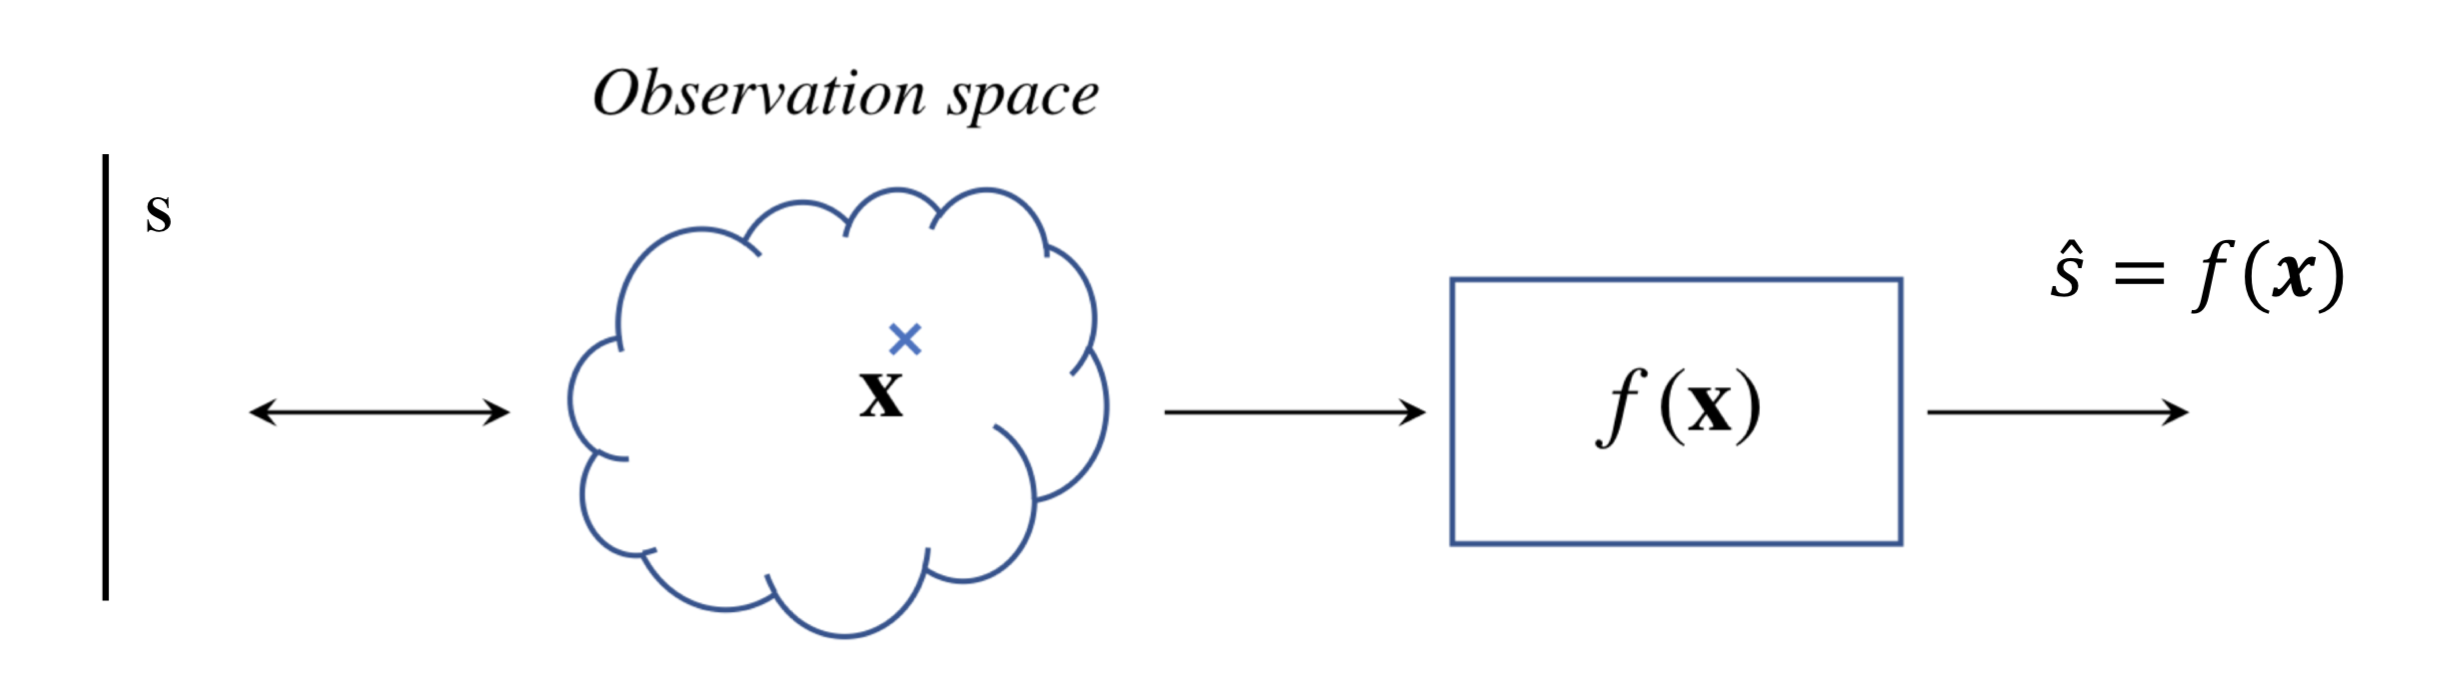
\includegraphics[width=10cm]{Figures//estimation_overview.png}
\end{center}
\caption{Diagram block of estimation problems.\label{fig:est_overview}}
\end{figure}

The estimator's performance is evaluated by how well $\hat{S}$ approximates $S$, typically using a predefined cost function that quantifies the estimation error. A well-designed estimator seeks to minimize the expected value of this cost.

There are two primary tasks in estimation problems:
\begin{itemize}
\item Analysis: given an estimator, assess its performance based on statistical criteria.
\item Design: find an estimator $f()$ that optimizes a predefined performance goal.
\end{itemize}
}

%%%%%%%%%%%%%%%%%%%%%%%%%%%%%%
\subsection{\textcolor{blue}{Probability model}}
\label{subsec:statistical_info}

The statistical relation between the observations and the target variable is described by the {\bf joint} probability density function (pdf) of ${\bf X}$ and $S$: $p_{{\bf X},S}({\bf x},s)$, or some distribution related to it. 

The joint pdf can be factorized as \textcolor{blue}{a product} of conditional and marginal pdfs:
\begin{align}
p_{{\bf X},S}({\bf x},s) = p_{{\bf X}| S}({\bf x}| s) \cdot p_S(s) 
                         = p_{S|{\bf X}}(s|{\bf x}) \cdot p_{\bf X}({\bf x}) 
\end{align}

In the context of estimation theory, these factors receive specific names:

%%%%%%%%%%%%%%%
\begin{itemize}
\item The {\bf likelihood} of $S=s$ for observation ${\bf x}$, $p_{{\bf X}|S}({\bf x}|s)$: it characterizes the generation of observations for each value of the target variable.
\item The {\bf prior (or \textit{a priori}) distribution}  of $S$, $p_S(s)$: it describes how much is known (or unknown) about the target variable before observing ${\bf X}$. 
\item The {\bf posterior (or \textit{a posteriori}) distribution} of $S$ given ${\bf X}={\bf x}$, $p_{S|{\bf X}}(s|{\bf x})$: it describes the knowledge (or the uncertainty) about $S$ after observing ${\bf X}$.
\item The {\bf evidence} or marginal distribution of ${\bf X}$, $p_{{\bf X}}({\bf x})$.
\end{itemize}
%%%%%%%%%%%%%

\textcolor{blue}{The information available to design the estimator may depend on the application. In some cases, the likelihood function is known, because it can be related to the physical generative process of the observations. If additionally}, a prior distribution is available, the design can be grounded on the posterior distribution $p_{S|{\bf X}}(s|{\bf x})$, which can be calculated by means of Bayes' Theorem,
\begin{equation}
p_{S|{\bf X}}(s|{\bf x}) 
	= \frac{p_{{\bf X},S}({\bf x},s)} {p_{\bf X}({\bf x})} 
	= \frac{p_{{\bf X}|S}({\bf x}|s) p_S(s)}
	       {\int p_{{\bf X}|S}({\bf x}|s') p_S(s') ds'}
\end{equation}


%%%%%%%%%%%%%%%%%%%%%%%%%%%%%%%%%%%%%%%%%%%%%%%%%%%
\subsection{Cost functions for estimation problems}
\label{subsec_funcion_coste}

The evaluation and design of an estimator require some objective criteria. In some cases, we will consider that this criterion materializes in the form of a {\bf cost function} whose value we seek to minimize. %We note, however, that there are design strategies that fall outside of this approach, such as the direct maximization of some probability function.

A cost function $c(s,\hat s)$ is any measure of the discrepancy between the target variable and the estimation. It is generally non-negative, $c(s,\hat s) \geq 0$, with equality for $s = \hat s$. \textcolor{blue}{Some cost functions} can be expressed as a function of the estimation error $e= s-\hat s$ and we will write\footnote{Note that the cost function is denoted with a lowercase letter, $c$, because it is a deterministic function, i.e., for fixed values of $s$ and $\hat s$ the cost always takes the same value. However, as with the estimation function, the application of that function to random variables will result in another random variable, i.e., $C = c(S,\hat S)$.} $c(s,\hat s) = c(s - \hat s) = c(e)$. Some examples are:
\begin{itemize}
\item \textcolor{blue}{Square error}: $c(e) = e^2$.
\item \textcolor{blue}{Absolute error}: $c(e) = |e|$.
\item Relative \textcolor{blue}{square} error: $c(s,\hat s) = \frac{(s-\hat{s})^2}{s^2}$
\item Cross Entropy: $c(s,\hat s) = - s \ln \hat s - (1-s) \ln (1-\hat s)$, for $s,\hat{s}\in [0,1]$
\end{itemize}

Since the target variable is unknown, the prediction cannot be computed by directly minimizing the cost $c(s, \hat s)$, and we have to work with expectations. The expected value of the cost is usually referred as the {\bf risk} of an estimator $\hat{s}=f({\bf x})$:
\begin{align}
\label{Est:coste_medio_gen}
R_f = \EE\{c(S,\hat S)\} 
    & = \int_{\bf x} \int_s c(s,f({\bf x})) p_{S,{\bf X}}(s,{\bf x}) ds d{\bf x}
\end{align}
By the Law of Large Numbers, this is the average cost we can expect from a given estimator, after a large number of predictions.

The {\bf conditional risk} is the conditional mean for a given observation
\begin{align}
\label{Est:cond_risk}
R(\hat s, {\bf x}) = \EE\{c(S, \hat s) |{\bf x}\} 
           & = \int_s c(s,\hat s) p_{S|{\bf X}}(s|{\bf x}) ds
\end{align}

%%%%%%%%%%%%%%%
\begin{example}[Evaluation of estimators 1]
\label{CalculoECM}
Given the joint distribution
\begin{equation}
p_{S,X}(s,x) = \left[
\begin{array}{ll}
\frac{1}{x}, & \qquad 0 \le s \le x ~~{\rm and}~ 0 < x \le 1 \\
0,           & \qquad \text{otherwise}
\end{array}
\right.,
\end{equation}
consider the estimators $\hat{S}_1 = \frac{1}{2}X$ and $\hat{S}_2 = X$. Which is the best estimator from the point of view of the \textcolor{blue}{square error}? To find out, we'll calculate the risk (i.e. the mean \textcolor{blue}{square error}) for both estimators.
Knowing that, for any $w$,
\begin{align}
R &=\mathbb{E}\{(S-wX)^2\}   
   = \int_0^1 \int_0^x (s-wx)^2 p_{S,X}(s,x) ds dx   
   = \int_0^1 \int_0^x (s-wx)^2 \frac{1}{x}ds dx   \nonumber\\
  &= \int_0^1 \left(\frac{1}{3} - w  + w^2 \right) x^2 dx  
   = \frac{1}{3}\left(\frac{1}{3} - w  + w^2 \right) 
\end{align}
Taking $w=1/2$ and $w=1$ we get, respectively, the risks
\begin{align}
R_1  = \EE\left\{(S-\hat{S}_1)^2\right\} 
	&= \EE\left\{\left(S-\frac12 X\right)^2\right\}   
     = \frac{1}{3}\left(\frac{1}{3} - \frac{1}{2}  + \frac{1}{4} \right)
     = \frac{1}{36} \\
R_2  = \EE\{(S-\hat{S}_2)^2\} & = \EE\{(S-X)^2\}   
 = \frac{1}{3}\left(\frac{1}{3} - 1  + 1 \right) = \frac{1}{9}
\end{align}
Therefore, from the point of view of the square error, $\hat{S}_1$ is a better estimator than $\hat{S}_2$.
\end{example}
%%%%%%%%%%%%%

%%%%%%%%%%%%%%%%%%%%%%%%%%%%%%%%%%%%%%%%%%%
\begin{example}[Evaluation of estimators 2]
Assume that $S$ is a random variable of mean 0 and variance 1, and $X$ is a noisy observation of $S$,
\begin{equation}
X = S + T
\end{equation}
where $T$ is a Gaussian random variable, independent of $S$, with mean $0$ variance $v$. We will compute the risk for the estimator $\hat{S} = X$ and different cost functions. For the \textcolor{blue}{square error}:
\begin{equation}
\EE\{(S-\hat{S})^2\} = \EE\{(S-X)^2\} = \EE\{T^2\} = v
\end{equation}
For the absolute error
\begin{align}
\EE\{|S-\hat{S}|\}
    &= \EE\{|T|\} 
     = \int_{-\infty}^{\infty} |t| \frac{1}{\sqrt{2\pi v}}\exp\left(-\frac{t^2}{2v}\right)dt 
\nonumber\\
    &= 2 \int_{0}^{\infty} t \frac{1}{\sqrt{2\pi v}}\exp\left(-\frac{t^2}{2v}\right)dt 
     = \sqrt{\frac{2v}{\pi}}
\end{align}
\end{example}
%%%%%%%%%%%%%%


%%%%%%%%%%%%%%%%%%%%%%%%%%%%%%
\subsection{Bias and Variance}
\label{subsec.bias_variance}

The performance of an estimator $\hat{S} = f(\mathbf{X})$ is often evaluated using two key quantities: \textit{bias} and \textit{variance}. These can be defined in both \textit{conditional} and \textit{unconditional} forms, depending on whether they are measured for a specific target variable or not.

%%%%%%%%%%%%%%%%%%
\begin{definition}[Conditional Bias]
The \textit{conditional bias} of an estimator $\hat{S}$ given that $S = s$ is defined as
\begin{align}
\text{bias}\{\hat{S} | S=s\} = \EE\{\hat{S} | S=s\} - s.
\end{align}
\end{definition}
%%%%%%%%%%%%%%%%

The conditional bias quantifies the expected deviation of the estimate from the true value of the target variable, $s$. 

The conditional \textbf{mean squared error (MSE)} of an estimator can be decomposed into its bias and variance components.

%%%%%%%%%%%%%%%%%%
\begin{theorem}[Bias-Variance decomposition]
For any estimator, $\hat{S}$ of random variable $S$, the conditional mean square error is
\begin{align}
\EE\{(\hat{S}-S)^2|S=s\} = {\rm bias}^2\{\hat{S} | S=s\} + {\rm var}\{\hat{S} | S=s\}
\end{align}
\end{theorem}
%%%%%%%%%%%%%


\begin{proof}

Since, for any random variable, $V$, $\EE\{V^2\} = \EE\{V\}^2 + {\rm var}\{V\}$, taking $V=S-\hat{S}$, and conditioning over $S=s$, we get
\begin{align}
\EE\{(\hat{S}-S)^2|S=s\} 
	&= \EE\{\hat{S}-S|S=s\}^2 + {\rm var}\{\hat{S}-S|S=s\}   \nonumber\\
	&= {\rm bias}^2\{\hat{S} | S=s\} + {\rm var}\{\hat{S}|S=s\} 
\end{align}
\end{proof}

This decomposition highlights the bias-variance tradeoff:
\begin{itemize}
\item Low-bias estimators tend to have high variance, leading to unstable predictions.
\item Low-variance estimators may introduce \textbf{bias} to improve stability.
\end{itemize}


Note that, in the above expressions, the bias, variance and mean square error are conditioned over a specific value of the target variable. We can extend these definitions to measures defined from unconditional means:

%%%%%%%%%%%%%%%%%%
\begin{definition}[Unconditional Bias]
The \textit{unconditional bias} of an estimator $\hat{S}$ of a random variable $S$ is
\begin{align}
\text{bias}\{\hat{S}\} = \EE\{\hat{S}\} - \EE\{S\}.
\end{align}
\end{definition}
%%%%%%%%%%%%%%%%

A similar unconditional bias-variance decomposition can obtained, that is given by
\begin{align}
\EE\{(\hat{S}-S)^2\} 
	&= \EE\{\hat{S}-S\}^2 + {\rm var}\{\hat{S}-S|S=s\}   \nonumber\\
	&= {\rm bias}^2\{\hat{S}\} + {\rm var}\{\hat{S}-S\} 
\end{align}

If $\text{bias}\{\hat{S} | S = s\} = 0$ for all $s$, the estimator is said to be \textit{conditionally unbiased}. If $\text{bias}\{\hat{S}\} = 0$, it is \textit{unbiased in the Bayesian sense}, meaning that its expected value matches the prior mean of $S$.


%Understanding both \textit{conditional} and \textit{unconditional} bias/variance is crucial when analyzing estimator performance, particularly when discussing the \textbf{Cramér-Rao Bound (CRB)} and the \textbf{Bayesian Cramér-Rao Bound (BCRB)}, where these distinctions play a key role.
